\section{Struttura centrale}

Lo sviluppo di un’applicazione segue un processo strutturato, articolato in diverse fasi. In fase di progettazione,
l'obiettivo principale è identificare le caratteristiche funzionali e comportamentali del sistema, delineando le componenti principali e le rispettive responsabilità.
Questa fase permette di definire un'architettura coerente, facilitando le successive scelte tecnologiche e implementative.\\
\\
Nella fase successiva, di implementazione, si procede con il passaggio dall’analisi teorica alla realizzazione concreta,
dove la selezione dell’architettura e delle tecnologie di riferimento assumono un ruolo centrale.
Le decisioni prese in questa fase determinano il comportamento dei diversi componenti e le modalità con cui essi interagiscono tra loro.
Un’attenta selezione delle soluzioni ottimali, più adatte ai requisiti definiti in fase di progettazione,
permette di impostare fin dalle prime iterazioni uno sviluppo efficiente e strutturato, minimizzando la necessità di revisioni successive.\\
\\
Mentre alcune decisioni risultano immediate o intercambiabili, altre richiedono analisi approfondite per individuare la soluzione più adatta.
Un approccio efficace consiste nello sviluppare inizialmente i componenti con requisiti ben definiti,
per poi affinare progressivamente l'integrazione e la configurazione degli altri elementi del sistema.
L'identificazione, anche parziale, di una struttura iniziale consente di delineare i vincoli di integrazione e di semplificare la definizione delle soluzioni residue.\\
\\
L’architettura dell’applicativo si basa su una chiara suddivisione in componenti, ciascuno con un ruolo specifico all’interno del sistema.
L'interfaccia grafica è responsabile della presentazione e dell’interazione con l’utente, ponendo particolare attenzione alla coerenza visiva e alla fluidità dell’esperienza.\\
\\
La logica applicativa viene gestita da un server centrale, il quale si occupa di coordinare le comunicazioni tra i diversi servizi e di garantire il corretto flusso delle operazioni.
La gestione dell’autenticazione degli utenti è delegata a un servizio apposito,
che consente di separare questa responsabilità dal resto del sistema, migliorando sia le prestazioni che la sicurezza.\\
\\
Un ulteriore aspetto fondamentale nella progettazione del sistema riguarda la protezione delle comunicazioni e dei dati sensibili.
L’adozione di misure di sicurezza adeguate è essenziale per garantire la protezione delle informazioni scambiate tra i vari componenti e
per ridurre i rischi derivanti da eventuali attacchi esterni.
Inoltre, per monitorare il corretto funzionamento dell’applicazione e identificare tempestivamente eventuali anomalie,
il sistema è integrato con strumenti di logging e analisi delle prestazioni.\\
\\
Questa organizzazione modulare consente di ottimizzare la scalabilità e la manutenibilità dell’applicativo,
facilitando eventuali evoluzioni future.
La suddivisione chiara delle responsabilità, unita a un’architettura flessibile e sicura,
rappresenta quindi un elemento chiave per garantire la stabilità e l’efficienza del sistema nel lungo periodo.\\
\\

\begin{figure}[h!]
    \centering
    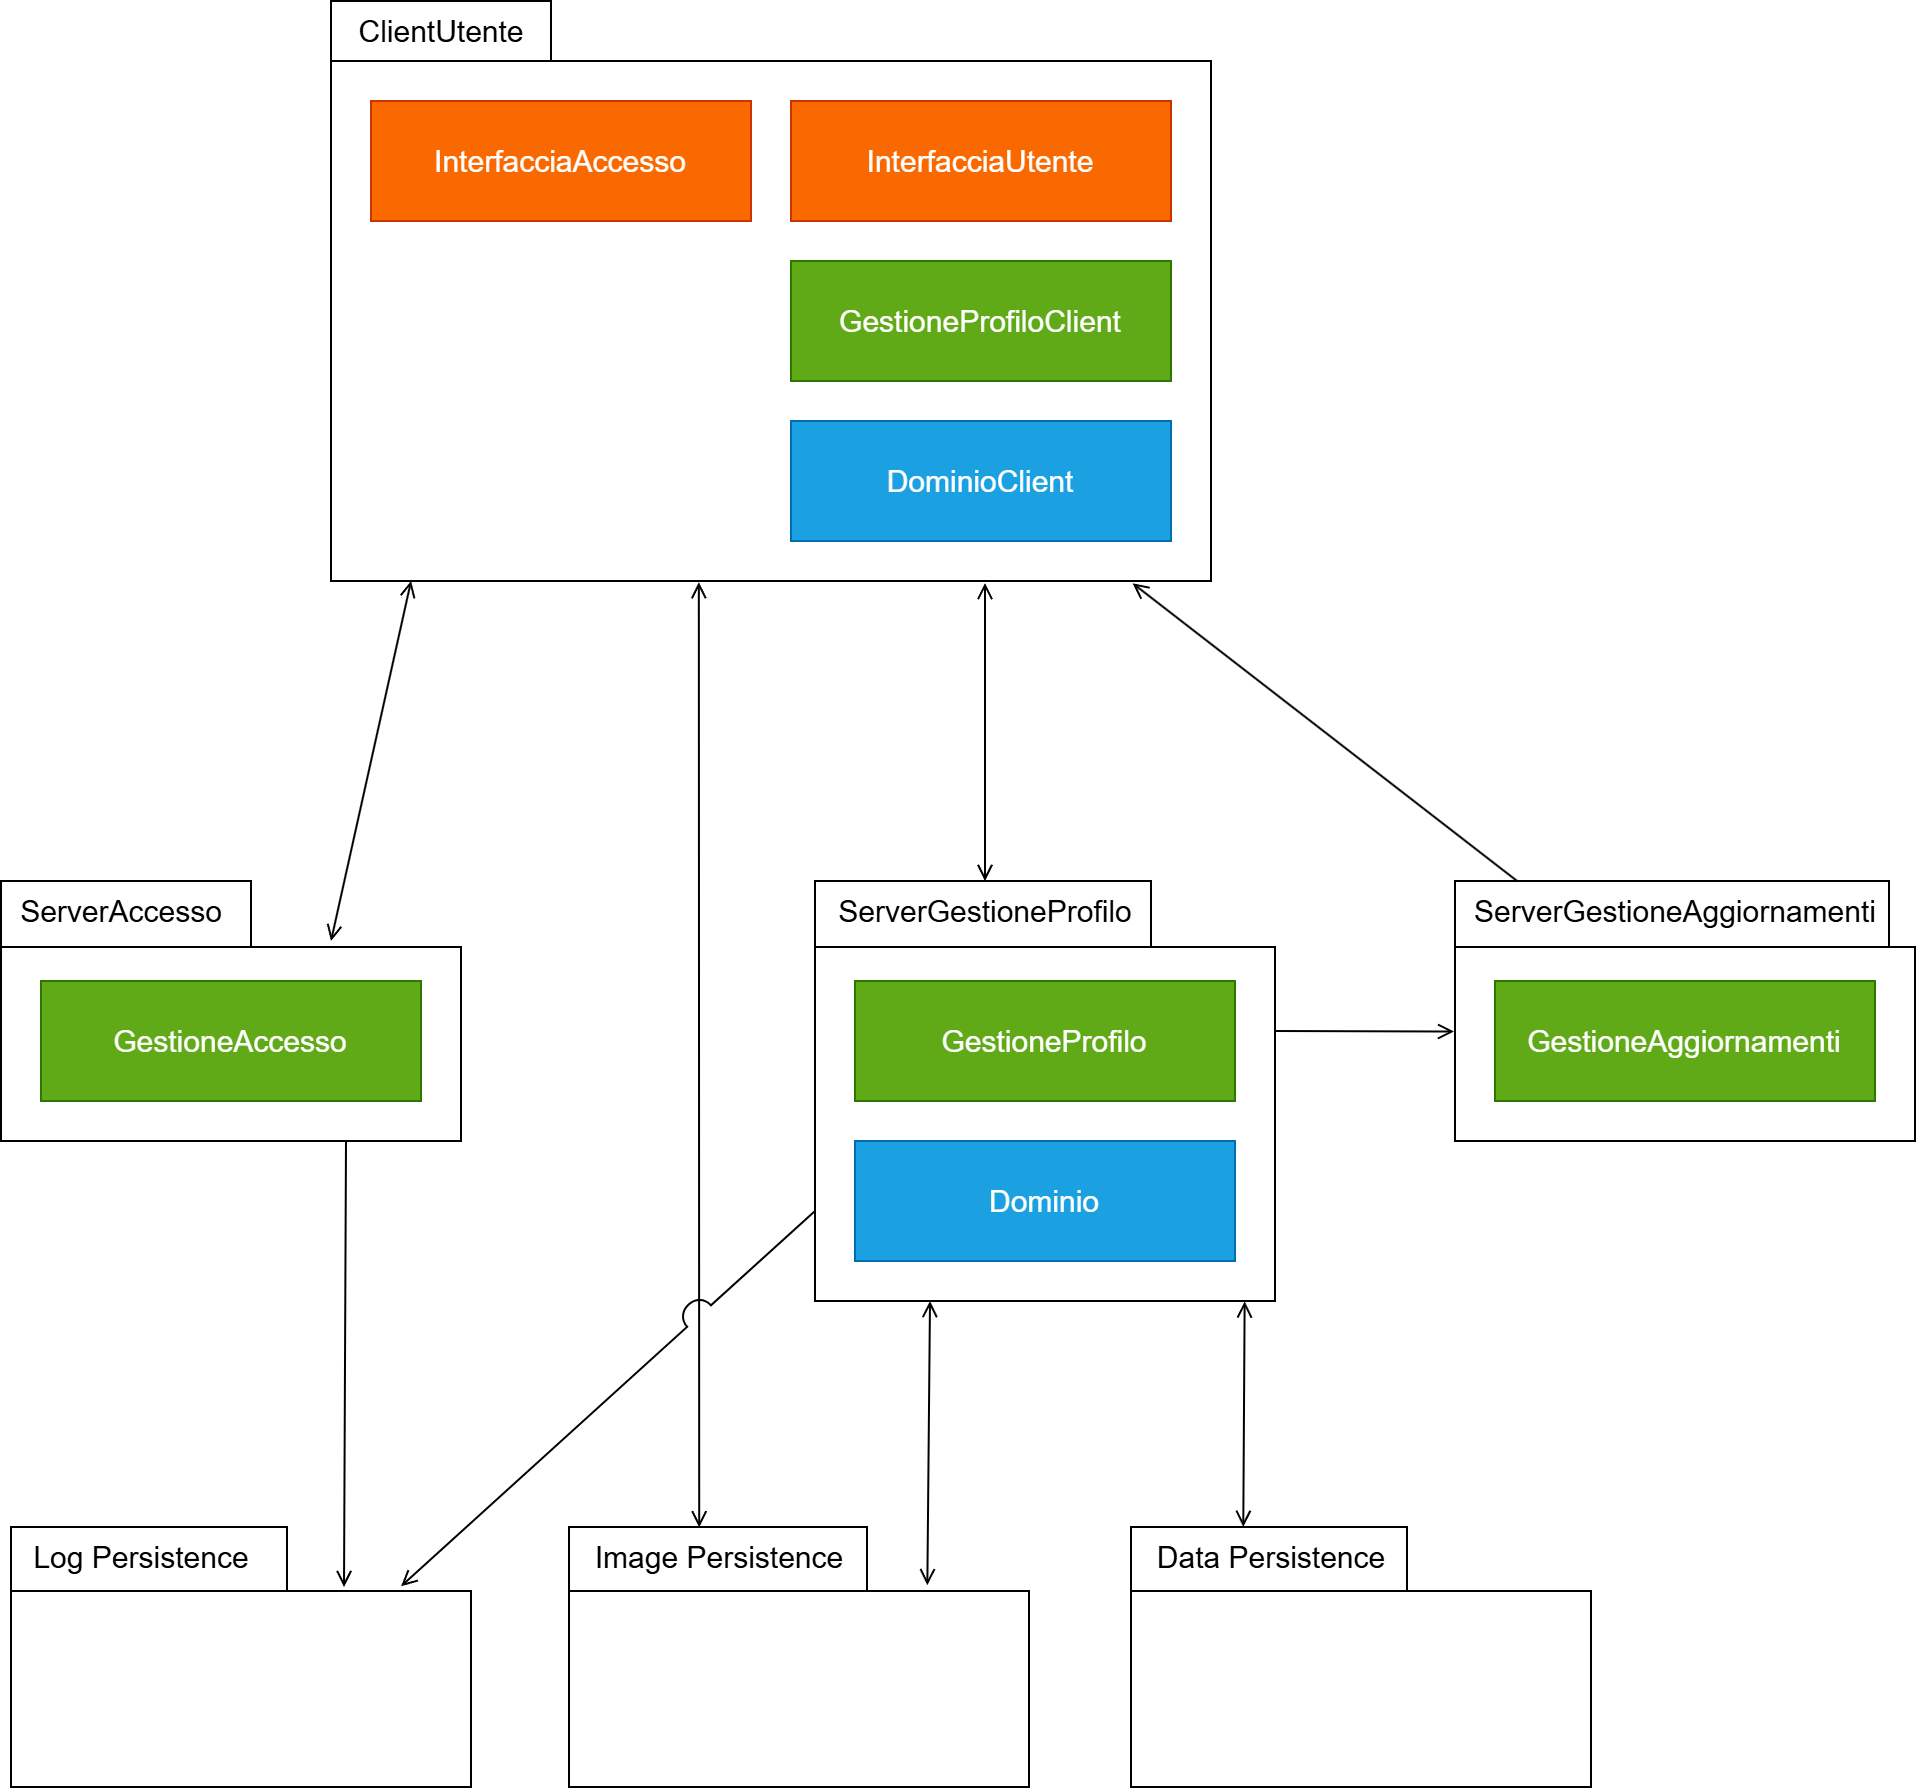
\includegraphics[width=\textwidth]{ProgettoDiagrammaPackage.png}
    \caption{Struttura e responsabilità delle parti del progetto}
\end{figure}

\clearpage
\subsection{Lo sviluppo del client}

L’utilizzo delle applicazioni per la gestione degli eventi può essere suddiviso in due fasi distinte, 
ciascuna con specifiche esigenze funzionali.\\
La prima fase riguarda infatti la pianificazione a lungo termine e l’organizzazione degli impegni.
In questa circostanza l’utente decide come distribuire il proprio tempo, pianificando attività e appuntamenti,
e strutturando il proprio calendario nel modo più efficiente per le proprie necessità.
La seconda fase riguarda invece la gestione degli eventi non ancora certi e definiti;
ciò include l’invito a un evento, l’eventuale conferma da parte dell’utente,
l’identificazione degli impegni a breve termine e l’aggiornamento del loro stato
(ad esempio, se l’evento sia ancora confermato, quante persone vi partecipano, se qualcuno ha annullato o se l'evento è già concluso)
con la gestione degli eventuali contenuti multimediali successivi all’evento. Queste due fasi implicano un approccio diverso da parte dell’utente,
comportando di conseguenza esigenze differenti a cui l’applicazione deve rispondere adeguatamente.\\
\\
Per rispondere a tali necessità, è fondamentale che l'applicazione offra un'interfaccia utente versatile, fruibile sia da desktop che da dispositivi mobili.
La versione desktop consente una pianificazione a lungo termine, offrendo una visione d'insieme chiara e completa di tutti gli impegni,
tale da facilitare la gestione del tempo.
D'altra parte, la versione mobile deve permettere una gestione rapida e dinamica degli eventi quotidiani,
garantendo che l'utente possa rimanere sempre connesso e aggiornato sugli sviluppi in tempo reale.\\
\\
Inoltre, considerando che l'applicazione è destinata a un utilizzo diffuso e a un'utenza potenzialmente elevata,
è necessario garantire tempi di risposta ridotti e una gestione efficiente delle richieste concorrenti.
Ciò implica la progettazione di un sistema in grado di scalare facilmente,
per supportare un ampio numero di utenti simultanei senza compromettere le prestazioni.\\
\\
\clearpage


\subsubsection{Il framework di sviluppo}
Al fine di ottenere tutte le prestazioni precedentemente elencate, la scelta è ricaduta sull’adozione del framework di sviluppo Flutter.
Diversi fattori motivano tale decisione. \\
In primo luogo, l'architettura di Flutter si basa su un motore grafico indipendente dalla piattaforma di esecuzione,
il che consente di ottenere elevate prestazioni e garantire un'esperienza utente uniforme su dispositivi diversi. \\
In secondo luogo, Flutter adotta un approccio dichiarativo nella progettazione dell'interfaccia grafica,
che facilita lo sviluppo di componenti reattivi attraverso un codice conciso, facilmente manutenibile.\\
\\
Un ulteriore vantaggio di Flutter è rappresentato dalla crescente adozione nel settore,
dalla solidità della community di sviluppo e dal supporto offerto da Google,
che ne assicurano la stabilità, l'efficienza, la sicurezza e la disponibilità di componenti personalizzabili per l'intero ciclo di vita del prodotto.
Infine, Flutter consente uno sviluppo rapido e interattivo grazie alla sua sintassi intuitiva e al meccanismo di hot reload,
che riduce significativamente i tempi di compilazione e facilita il testing in tempo reale.\\
\\
Tra le altre tecnologie valutate per lo sviluppo dell'interfaccia grafica, vi erano React Native e Xamarin.
Tuttavia, entrambe presentano alcune limitazioni: 
le applicazioni finali sviluppate con React Native tendono ad avere dimensioni più elevate e le prestazioni risultano inferiori,
in particolare nella gestione della memoria.
Xamarin, pur essendo una valida opzione, presenta una curva di apprendimento più ripida e 
una comunità di sviluppatori ridotta rispetto a Flutter,
con una conseguente minore disponibilità di componenti e librerie.\\
\\
Per quanto Flutter consenta di uniformare l'esperienza utente su dispositivi diversi e semplifichi la compilazione per le varie piattaforme,
alcune configurazioni rimangono comunque dipendenti dalla tecnologia su cui l'applicazione viene eseguita.
Di conseguenza, ciascun eseguibile richiede una manutenzione aggiuntiva, inclusi gli aggiornamenti delle dipendenze specifiche,
sia a livello di deployment che di gestione delle versioni.\\
\\

In una fase iniziale dello sviluppo, nell'ottica di coprire il più ampio mercato possibile con il minor numero di piattaforme,
si è deciso di sviluppare una versione fruibile via web e una per dispositivi Android.\\
\\
\subsubsection{L'implementazione}
\clearpage
\subsubsection{La distribuzione}

Già consolidata e affidabile, sin dalle prime fasi di sviluppo del progetto è stata adottata la piattaforma cloud Azure, per garantire un'infrastruttura solida e scalabile.\\
\\
Nell'ambito delle tecnologie offerte da Azure per la  distribuzione del codice web, si è scelto Azure Static Web App, un servizio di hosting progettato per applicazioni web statiche. \\
\\
La preferenza per questa soluzione è derivata dalla affidabilità dell'infrastruttura di Azure e dai bassi costi operativi per un utilizzo limitato,
fattori che la rendono particolarmente vantaggiosa.\\
\\
Questa selezione è stata resa possibile in quanto l’interfaccia sviluppata non prevede la creazione dinamica di contenuti,
ovvero la pagina che viene restituita rimane invariata indipendentemente dall’utente che effettua la richiesta.
I dati specifici dell’utente verranno infatti richiesti ad un server terzo (qualora non siano già presenti in una cache locale).
Questa scelta consente di rendere l’interfaccia grafica completamente indipendente dall’identità dell’utente,
migliorando così le prestazioni e riducendo il carico computazionale delegato a Azure Static Web App.\\
\\
Inoltre, in attesa della pubblicazione dell’applicazione sull’App Store di Android, l’eseguibile è stato temporaneamente reso disponibile tramite Azure Storage Container.
Questo servizio consente l’archiviazione e la distribuzione di file di varie tipologie, fornendo un link diretto per il recupero.\\


\clearpage
\begin{figure}[h!]
    \begin{center}
        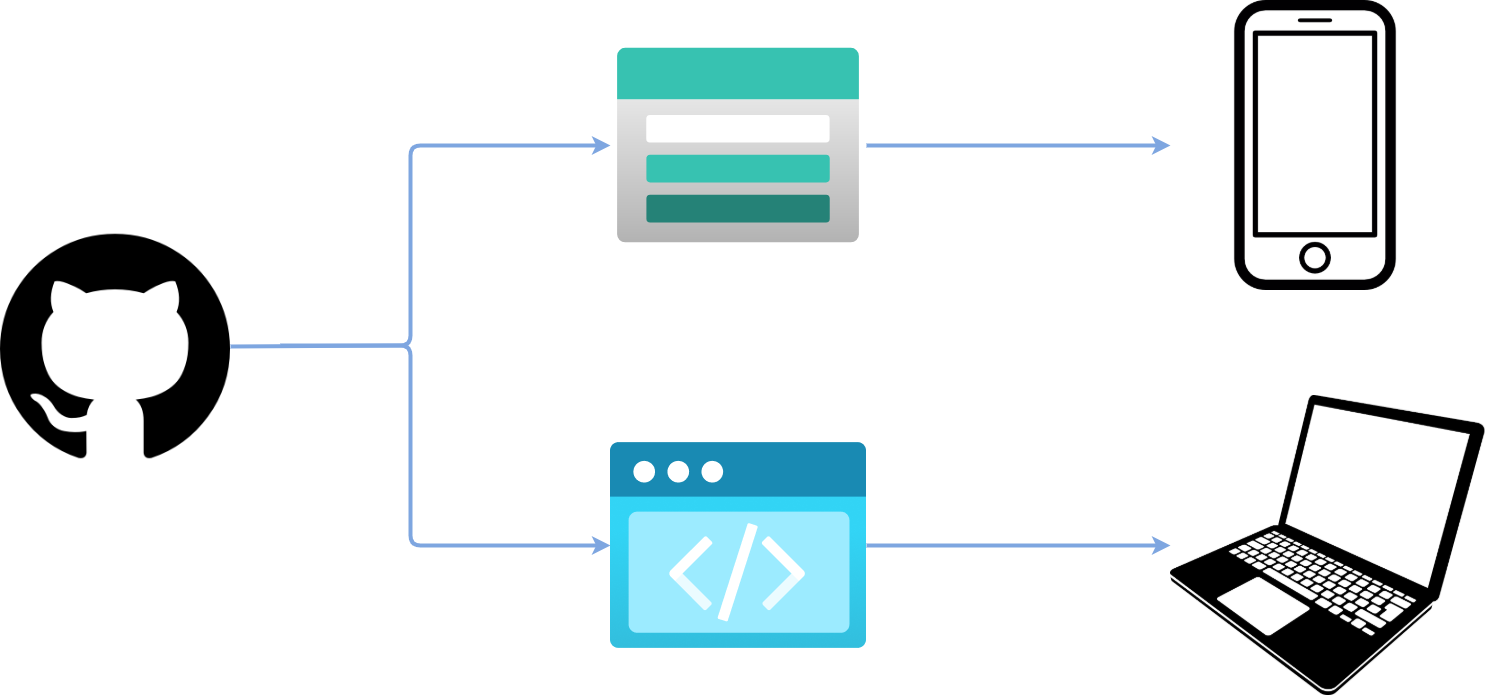
\includegraphics[height=0.28\textheight]{DeployFront.png}
        \caption{Diagramma di aggiornamento e distribuzione del client}
    \end{center}
\end{figure}

\subsubsection{L'aggiornamento}
Per garantire un processo di aggiornamento efficiente e automatizzato,
sia il codice distribuito sulla web app che l’applicativo ospitato nel container vengono gestiti tramite GitHub Actions,
che ne assicura l’aggiornamento automatico a ogni nuova versione. \\
\\

Nella fruizione tramite browser, il codice si aggiorna automaticamente a ogni accesso, mentre per l’applicativo su dispositivo mobile è necessaria una reinstallazione manuale.
Per questa ragione, gli utenti dell’applicazione verranno notificati tempestivamente ogni volta che sarà disponibile una nuova versione.\\
\\
\clearpage
\subsection{L’architettura del server principale}

Per poter essere in grado di gestire un numero elevato di richieste in tempi ridotti, l’applicazione deve garantire un’elevata scalabilità.\\
\\
Capace di soddisfare al meglio questa esigenza è Azure Functions, un servizio serverless che consente di suddividere il codice in unità indipendenti,
ciascuna eseguita in un ambiente di esecuzione unico per ogni richiesta.
Questa caratteristica, combinata con la virtualizzazione dell’ambiente di esecuzione offerta dal cloud, consente una scalabilità potenzialmente illimitata.\\
\\
L’indipendenza e la natura stateless di ogni funzione, ovvero la sua esecuzione svincolata dalle informazioni sullo stato o sulla sessione, sono responsabilità dello sviluppatore.
Ogni funzione segue il principio di singola responsabilità, eseguendo un unico compito specifico.
Tuttavia, nel caso di richieste che necessitino l’esecuzione coordinata di più funzioni, Azure Durable Functions fornisce una soluzione efficace.\\
\\
Integrata all’interno delle Azure Functions, Azure Durable Function consente la creazione di una funzione orchestrator,
incaricata di gestisce l’ordine, lo stato, il ciclo di vita e le risposte delle varie funzioni coinvolte nell’elaborazione della richiesta.\\
\\
Mantenendo un'architettura indipendente e scalabile, questa soluzione consente di gestire efficacemente scenari in cui un’esecuzione sequenziale delle operazioni è cruciale,
dove è necessario effettuare tentativi aggiuntivi in caso di errore o fallimento o si richiede l'attesa del completamento di operazioni con un tempo di esecuzione prolungato.\\
\\
Tuttavia, l'architettura stateless e l’accoppiamento debole tra orchestrator e funzioni in esecuzione causano un tempo di risposta delle Azure Durable Functions più elevato.
Per ottimizzare l’allocazione delle risorse, il sistema avvia perciò solo le funzioni strettamente necessarie all’esecuzione del compito determinato,
stanziando al minimo il consumo computazionale.\\
\\

\subsubsection{La scelta del linguaggio}
Come linguaggio di programmazione per lo sviluppo delle funzioni è stato utilizzato C\#.
La consapevolezza che sia l’ambiente di sviluppo di C\#, ovvero il framework .Net, sia la piattaforma Azure siano entrambi sviluppati e mantenuti dalla stessa azienda, Microsoft,
garantisce elevati livelli di stabilità, supporto e coordinamento delle tecnologie adottate.\\
\\
L’integrazione con Entity Framework Core permette la mappatura direttamente in oggetti dei componenti del dominio, 
semplificando così la logica delle relazioni e astraendo le comunicazioni con il database.
Grazie all’utilizzo delle proprietà virtuali degli oggetti si può applicare il lazy loading, 
riducendo il numero di richieste al database solo a quando esse sono strettamente necessarie, mantenendo in codice a livello logico ed ottimizzandone le prestazioni.
\subsubsection{Lo sviluppo}
Lo sviluppo è stato condotto utilizzando Visual Studio Code, piattaforma che, grazie ad apposite estensioni,
consente un collegamento diretto ai servizi cloud Azure, semplificando il processo di aggiornamento del codice, rendendolo estremamente lineare ed immediato.\\
\\
Azure Function in ambiente .Net supporta due modelli di esecuzione e sviluppo: in-process worker o isolated worker.
Il worker è il processo all’interno dell’applicativo che gestisce la creazione delle risorse e l’esecuzione delle funzioni in risposta alle richieste.
Nella modalità in-process, la funzione viene eseguita all’interno dello stesso processo del worker che l’ha generata,
riducendo la quantità di allocazione delle risorse necessarie ma condividendo l’ambiente di esecuzione.
Nel modello isolated, invece, ogni funzione viene eseguita attraverso un processo indipendente dedicato,
garantendo maggiore isolamento e quindi riducendo le possibili dipendenze tra le funzioni. \\
\\
Inoltre, il modello isolated worker offre ulteriori vantaggi, grazie al maggiore supporto fornito:
innanzitutto esso prevede una maggiore compatibilità, grazie al più ampio numero di versioni del framework .Net,
a differenza del modello in-process, limitato alle sole versioni con supporto a lungo termine.
In secondo luogo, il supporto per la creazione di middleware personalizzati 
permette l’elaborazione di un codice intermedio tra la chiamata e l’esecuzione della funzione,
funzionalità invece non disponibile nel modello in process.
Considerati questi vantaggi, le funzioni sono state sviluppate utilizzando il modello isolated worker 
per garantire maggiore flessibilità, compatibilità e modularità dell’architettura.
\clearpage





\subsection{Autenticazione}


Poiché la modalità di autenticazione rappresenta un elemento cruciale per l’esperienza dell’utente, 
in quanto deve assicurare un accesso sicuro all’applicazione mantenendone la semplicità, la facilità del processo autenticazione deve essere garantita.
Offrire agli utenti la possibilità di autenticarsi tramite il proprio authentication provider di fiducia migliora sicuramente l’usabilità e l’apprezzamento degli utenti, 
ma è altrettanto essenziale consentire la possibilità di creare account dedicati esclusivamente all’applicazione.
Di conseguenza, il sistema di gestione degli accessi deve supportare sia la registrazione e la gestione autonoma degli account specifici per il servizio, 
sia fornire l'integrazione con provider di autenticazione esterni.\\
\\
Per lo scopo, Azure fornisce Microsoft Entra ID, parte della suite di servizi di autenticazione e autorizzazione Microsoft Entra. 
Sebbene teoricamente in grado di soddisfare i requisiti sopra indicati, 
la complessità della documentazione e le difficoltà riscontrate nell’integrazione con il servizio dell’applicativo
 hanno portato a valutare soluzioni alternative negli ambienti cloud.\\
\\
La scelta è ricaduta su Firebase Authentication, che garantisce sia la possibilità di creare account dedicati che di collegarsi attraverso altri authentication providers. 
Inoltre, la piattaforma presenta un’interfaccia chiara e offre servizi di integrazione di facile utilizzo sia tramite Flutter che tramite C\#.
Dal punto di vista economico, il servizio risulta vantaggioso, essendo gratuito fino ai cinquantamila utenti mensili attivi.\\
\\
Uno dei requisiti fondamentali del progetto prevede che ogni account sia associato in modo univoco a un singolo utente. 
Durante la fase di creazione del profilo, tuttavia, l’account viene inizialmente registrato nel database gestito da Firebase. 
Pertanto, al primo accesso, il server, dopo aver verificato l’autenticità della richiesta, provvede a creare una copia dell’account, 
generando poi il relativo nuovo oggetto utente e il primo profilo associato.\\
\clearpage
\begin{figure}[h!]
    \centering
    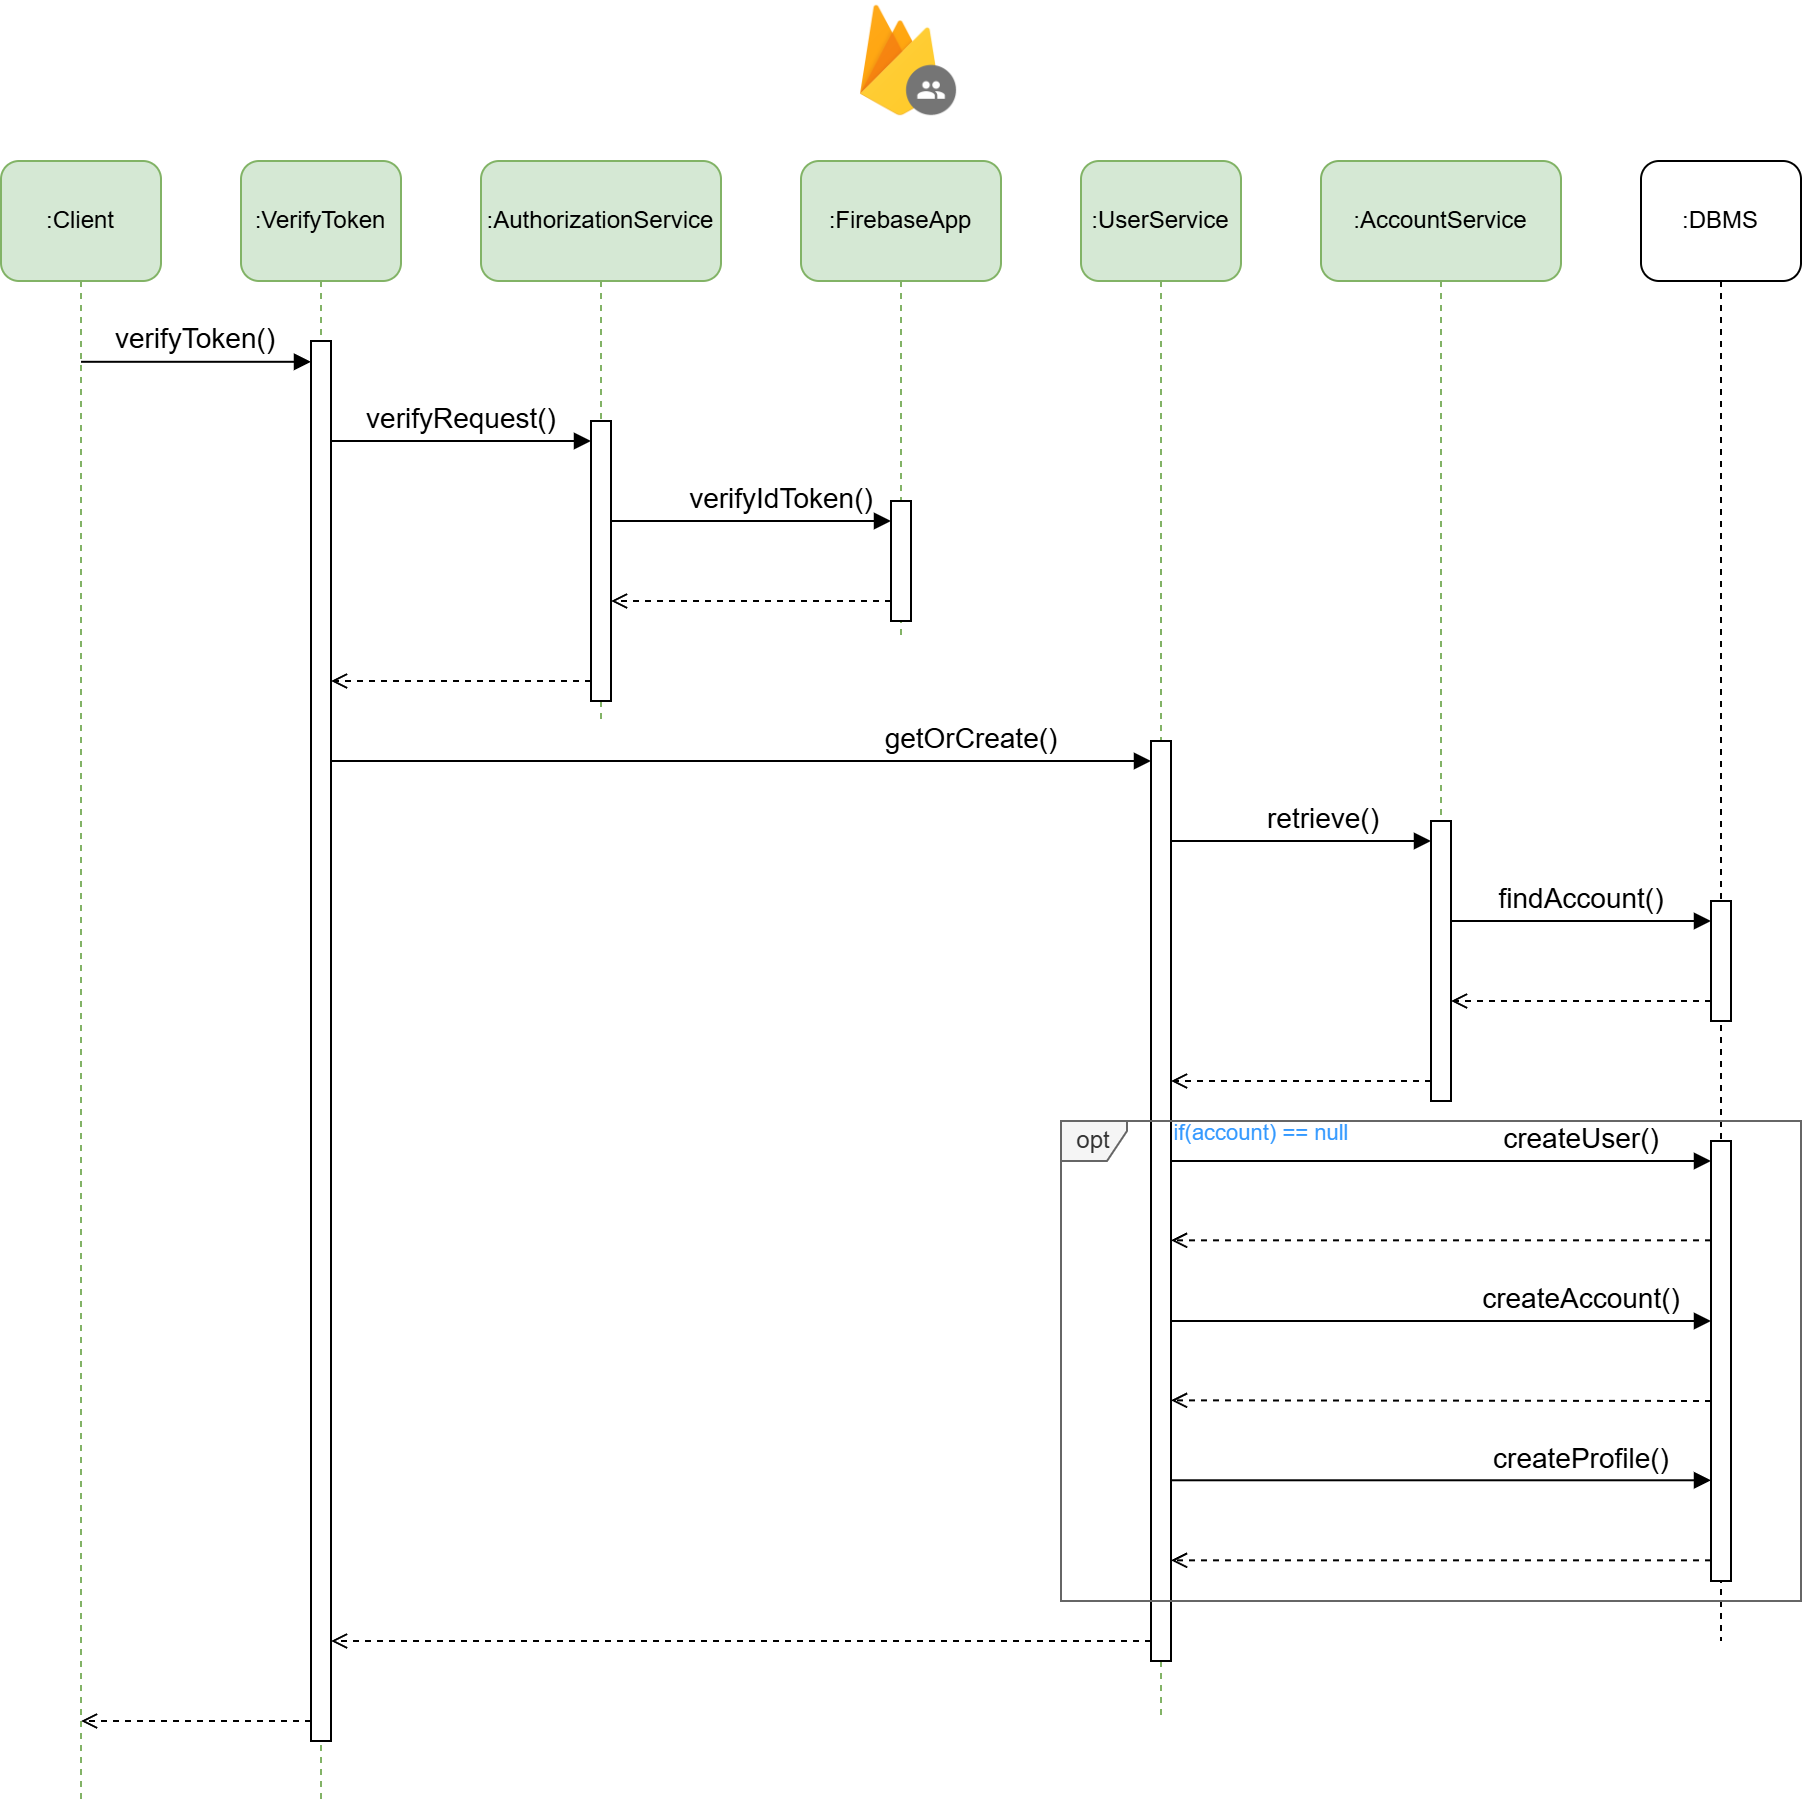
\includegraphics[width=\textwidth]{IIVerifyToken2.png}
    \caption{Diagramma di sequenza per la creazione di un account}
\end{figure}
Per garantire un processo di autenticazione sicuro ed efficiente, a ogni richiesta che richiede identificazione, 
il dispositivo utente aggiunge anche il token di autenticazione, salvato durante il primo accesso e la verifica iniziale. 
Il server verifica quindi la validità del token prima di procedere con l'esecuzione della richiesta.

\clearpage
\subsection{La sicurezza}

Il collegamento tra i vari componenti all’interno dell’ambiente Azure richiede l’utilizzo di chiavi e stringhe di connessione. 
Il salvataggio di tutte le chiavi sensibili è stato affidato al servizio Azure Key Vault,
 un server che permette la centralizzazione dei dati, cifrando il contenuto e garantendo un controllo maggiore sul loro utilizzo. 
Quando necessario i servizi, in particolare le Azure Function, contatteranno il Key Vault per l’ottenimento delle chiavi necessarie, 
riducendo il rischio di un’intercettazione data magari da un errore durante lo sviluppo.\\
\\
Le comunicazioni tra i vari componenti devono avvenire in sicurezza, garantendo autenticità e confidenzialità. 
Per questo motivo tutte le comunicazioni tra dispositivi client e i vari servizi utilizzano la tecnologia TLS, che permette di cifrare i messaggi grazie ad uno standard collaudato. 
In particolare, le comunicazioni tra i client e Azure Function, così come con Firebase Authentication e il server per la persistenza delle immagini, 
avvengono tramite protocollo HTTPS, mentre le comunicazioni con il server per gli aggiornamenti in tempo reale usano il protocollo WSS.\\
\\
L’accesso al database è ristretto alle sole risorse Azure, garantendo l’isolamento dall’esterno, che comprometterebbe altrimenti l’affidabilità dei dati.\\
\\
Infine, l’identificativo di ogni elemento del dominio è nascosto all’utente tramite la creazione di codici hash univoci 
che permettono comunque l’identificazione dell’oggetto senza rivelare ulteriori informazioni. 
In particolare, il caricamento delle immagini avviene grazie ad un link univoco dato dalla combinazione degli identificativi dell’evento e dell’immagine. 
Utilizzando i codici di hash diventa molto complicato il ritrovamento delle immagini senza essere a conoscenza dei codici, 
che non avendo natura incrementale ma distribuita rende indovinare un link valido.

TODO Dos e limite alle dimensioni delle richieste

\clearpage
\subsection{Monitoraggio}

Il monitoraggio del sistema è attuato in due modalità: tramite salvataggio dei log e controllo delle prestazioni del sistema.\\
\\

Relativamente a Firebase Authentication vengono forniti con il servizio sia le interfacce
per il controllo delle prestazioni che la gestione dei log. Non è quindi richiesta alcuna ulteriore azione.\\
\\
Per monitorare le Azure Functions sarà invece necessario collegare Azure Application Insights, servizio che provvede a controllare il funzionamento e la risposta del servizio. 
Una volta unito il servizio, infatti, Azure Application Insight permette la presentazione e l'analisi di numerose metriche, quali il tempo di risposta e il consumo di risorse. 
Consente inoltre di testare la risposta dell’applicativo simulando diversi scenari e riassumendo il loro comportamento.\\
\\
La creazione dei log è invece delegata al programmatore, in quanto è necessario integrarli nel codice. 
Nel momento della creazione, ogni funzione riceve, tramite dependency injection, un servizio Logger che permette la creazione e il salvataggio dei log. 
Tali log saranno poi consultabili e analizzabili tramite l’interfaccia fornita da Azure Application Insight.\\
\\
\clearpage